\chapter{Tatanan Sistem Saraf}\label{ch:b3:nervous-systems}

Seekor ubur-ubur punya beberapa ribu neuron di dalam sebuah jala tanpa pusat
dan dapat berenang, makan, serta menegakkan dirinya. Seekor gurita punya
setengah miliar, dua pertiganya di dalam lengannya, yang masing-masing dapat
menyelesaikan sebuah masalah yang tidak diberitahukan kepada otaknya. Anda punya
delapan puluh enam miliar, yang disambung seratus triliun sinapsis, yang
berjalan pada dua puluh watt --- seperlima tenaga Anda bagi dua persen massa
Anda --- dan Santiago Ramón y Cajal, yang menggambarnya sel demi sel pada
dasawarsa 1890-an dari irisan yang diwarnai perak, melihat bahwa mereka sel
terpisah yang bersentuhan tanpa melebur dan bahwa isyarat mengalir melewatinya
dalam satu arah. Jilid sebelumnya memperlakukan neuronnya: potensial istirahatnya,
potensial aksinya, sinapsisnya. Bab ini memperlakukan neuron itu dirangkai
menjadi apa: kabel pasif yang membatasi seberapa jauh sebuah isyarat menyebar dan
seberapa cepat, sirkuit --- refleks, pengayun, penghambatan sekeliling ---
yang darinya tingkah laku dirakit, denah sistem saraf vertebrata dan \omterm{def:b3:nervous-systems:cells}{glia} yang
menjaganya tetap berjalan, anggaran tenaganya, serta cara hewan yang berbeda
menyebarkan neuronnya.

\section{Neuron dan glia}

\begin{definition}[Sel sistem saraf]\label{def:b3:nervous-systems:cells}
\index{neuron!jenis}\index{glia}\index{astrosit}%
\index{oligodendrosit}\index{mielin}\index{mikroglia}\index{interneuron}
Neuron hadir dalam beberapa arsitektur yang berulang di seluruh otak:
sel \emph{piramidal}, yakni neuron proyeksi pemacu korteks,
dengan sebuah dendrit apikal yang panjang dan sebuah akson yang dapat mengembara
semeter; sel \emph{Purkinje} \omterm{def:b3:nervous-systems:plan}{otak kecil}, yang pohon dendritnya
yang pipih menerima dua ratus ribu sinapsis; neuron indra dengan satu
juluran ke tepi dan satu ke sumsumnya; serta \emph{interneuron},
yakni sel berakson pendek yang tinggal di dalam sebuah daerah, kebanyakan bersifat
menghambat. Sekitar empat dari lima neuron korteks melepaskan glutamat lalu
memacu; satu dari lima melepaskan GABA lalu menghambat. \emph{Glia}, yang
sebanyak neuronnya, mengerjakan selebihnya. \emph{Astrosit} membungkus sinapsis
dan pembuluh darah: mereka mengambil kalium yang dilepaskan neuron yang menyala
dan glutamat yang ditumpahkan sinapsis, memasok laktat, mengatur aliran darah
setempat, lalu memicu dan memelihara penghadang darah--otak.
\emph{Oligodendrosit} di dalam sistem saraf pusat dan \emph{sel Schwann}
di tepi membungkus akson dengan \emph{mielin}, yakni berlusin-lusin lapis
selaput yang mengisolasi aksonnya di antara simpul tempat salurannya
duduk. \emph{Mikroglia} adalah \omterm{def:b3:innate-immunity:innate}{makrofag} penghuni otaknya, yang memangkas
sinapsis pada perkembangan dan membersihkan puing. Sel ependima melapisi
bilik otaknya lalu membuat \omterm{prop:b3:nervous-systems:barrier-budget}{cairan serebrospinal}.
\end{definition}

\begin{proof}[Bukti eksperimental]
Pewarna perak kromat Golgi (1873) menghitamkan, karena alasan yang belum
diketahui, sekitar satu neuron dari seratus, seluruhnya, sambil membiarkan
selebihnya tak terlihat --- sehingga sebuah sel tunggal dapat dilihat utuh di
dalam kekusutan berjuta-juta. Golgi membaca sediaannya sendiri sebagai sebuah
retikulum sinambung; Cajal, sejak 1888, dengan memakai pewarna yang sama pada
jaringan embrio yang selnya lebih sederhana, melihat bahwa tiap selnya berakhir
dengan bebas, bahwa dendrit dan aksonnya berbeda, dan bahwa aksonnya berakhir
pada dendrit dan badan sel lain tanpa menyambunginya. Dari susunan sel indra dan
sel motorik ia menyimpulkan arah alirannya --- dendrit ke badan ke akson ---
yakni \emph{hukum pengkutuban dinamis}. Sherrington menamai celahnya
\emph{sinapsis} pada tahun 1897; mikroskop elektron menunjukkannya pada 1954.
\end{proof}

\begin{omfigure}
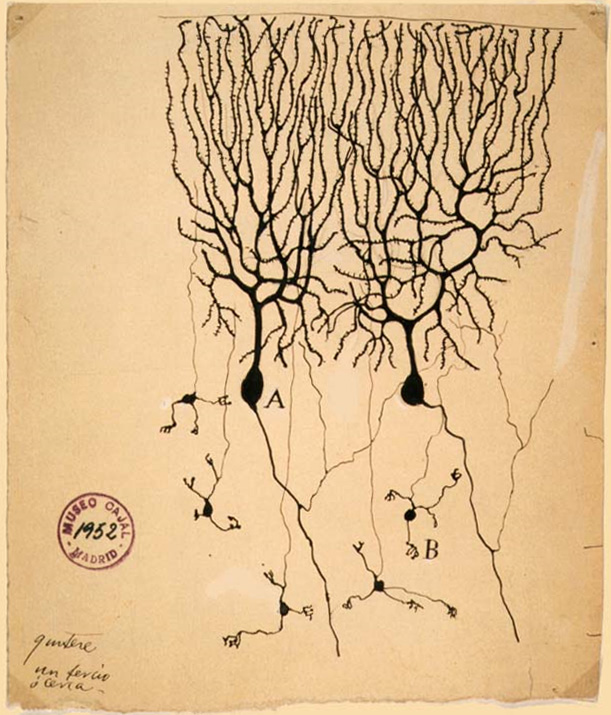
\includegraphics[width=0.30\linewidth]{images/book5/cajal-purkinje.jpg}\hspace{0.04\linewidth}
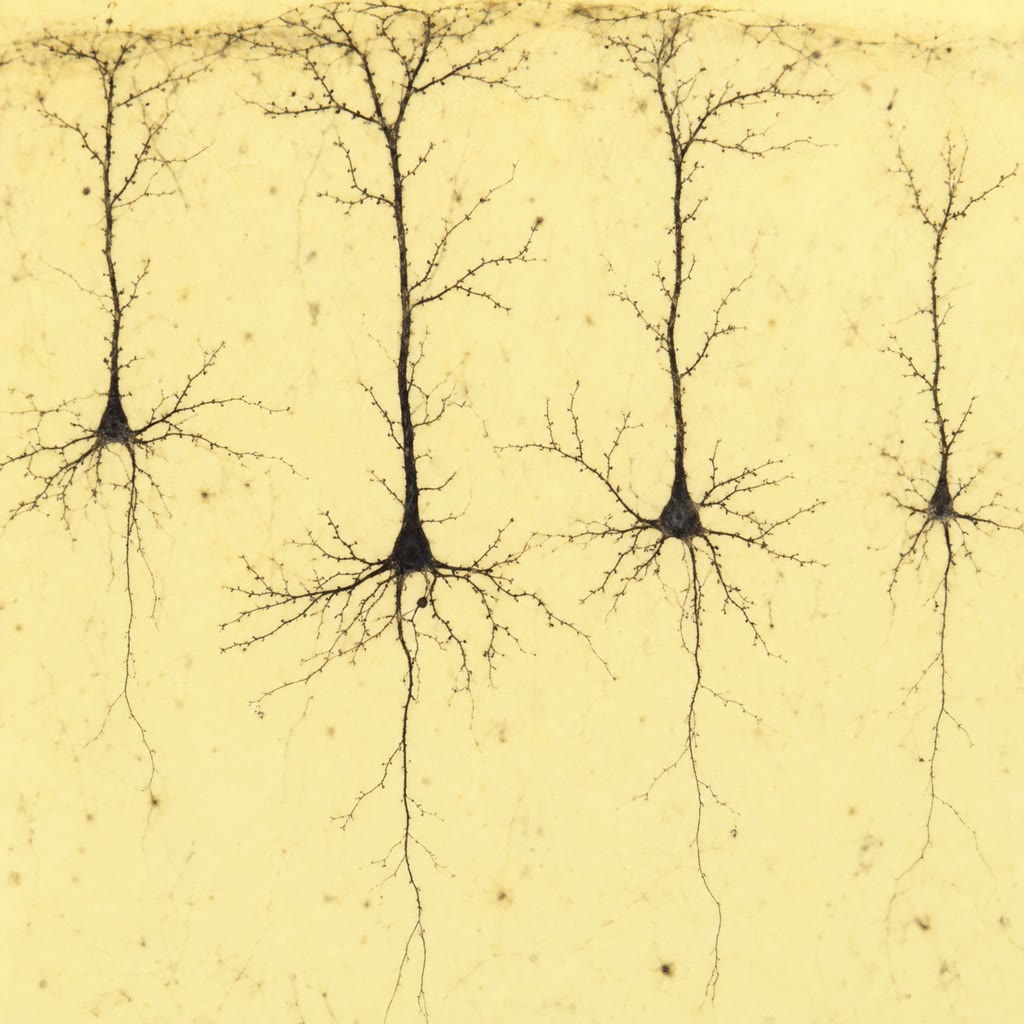
\includegraphics[width=0.30\linewidth]{images/book5/ai/b5-17-cortex-neurons.jpg}\hspace{0.04\linewidth}
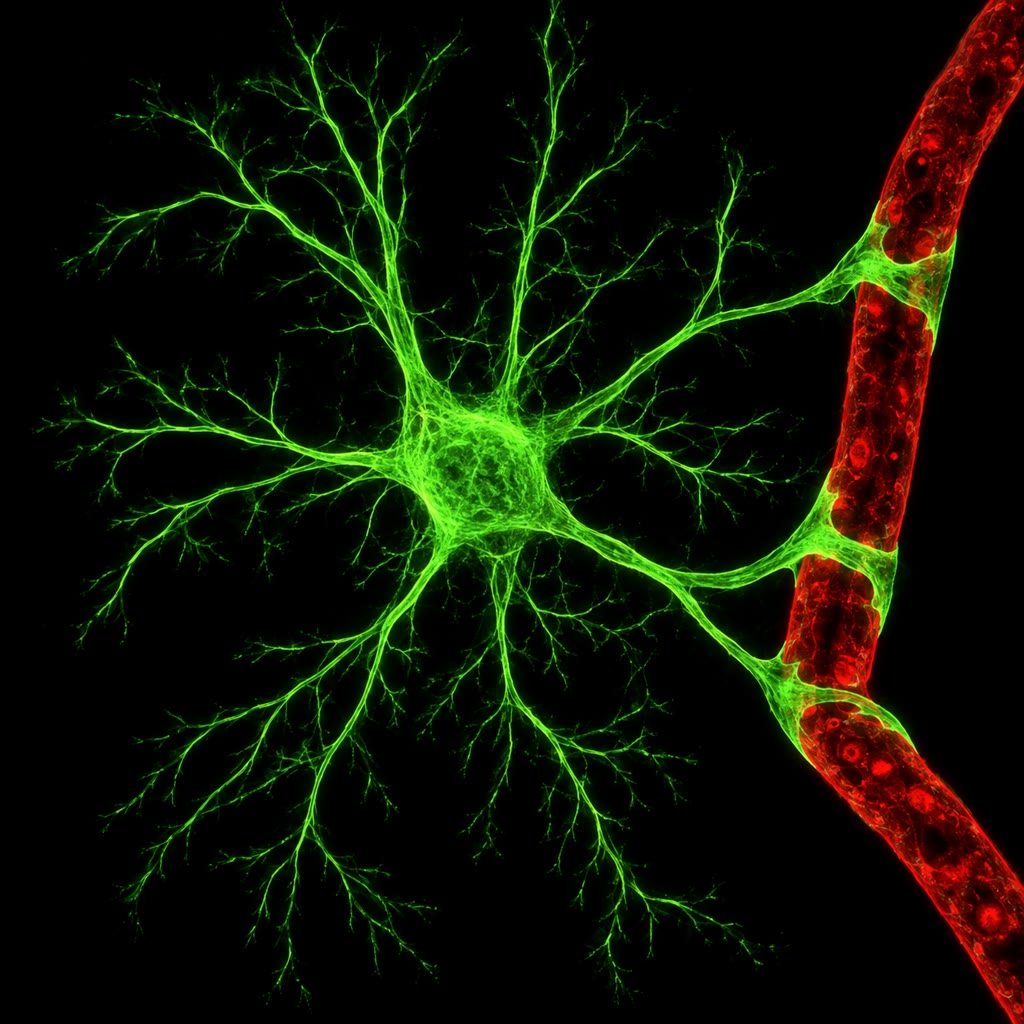
\includegraphics[width=0.30\linewidth]{images/book5/ai/b5-17-astrocyte.jpg}

{\small Kiri: sebuah sel Purkinje \omterm{def:b3:nervous-systems:plan}{otak kecil} yang digambar Cajal (1899)
dari sebuah irisan berpewarna Golgi --- seluruh pohon dendrit satu sel,
yakni hujah bagi neuron sebagai sebuah satuan (domain publik). Tengah:
neuron piramidal korteks dalam sebuah pewarnaan Golgi. Kanan: sebuah \omterm{def:b3:nervous-systems:cells}{astrosit}
(hijau) dengan kaki ujungnya pada sebuah kapiler (merah).}
\end{omfigure}

\section{Neuron sebagai sebuah kabel}

\begin{theorem}[Persamaan kabel keadaan mantap]\label{thm:b3:nervous-systems:cable}
\index{persamaan kabel}\index{tetapan panjang}%
\index{tetapan waktu!selaput}\index{laju hantaran}
Modelkanlah sebuah dendrit atau akson tak bermielin sebagai sebuah silinder
bergaris tengah $d$ yang sitoplasmanya beresistivitas $R_{i}$ dan selaputnya
beresistans jenis $R_{m}$ (resistans kali luas) dan berkapasitans $C_{m}$ tiap
luas. Tiap satuan panjang, resistans aksialnya $r_{i} = 4R_{i}/\pi d^{2}$
dan resistans selaputnya $r_{m} = R_{m}/\pi d$. Sebuah tegangan tetap
$V_{0}$ yang dikenakan pada $x = 0$ menyebar sepanjang seratnya sebagai
\[
V(x) = V_{0}\,e^{-x/\lambda}, \qquad
\lambda = \sqrt{\frac{r_{m}}{r_{i}}} = \sqrt{\frac{R_{m}\,d}{4R_{i}}},
\]
dengan $\lambda$ adalah \emph{\omterm{thm:b3:nervous-systems:cable}{tetapan panjang}}: yakni jarak yang sepanjangnya
sebuah isyarat pasif turun menjadi $1/e$, yang tumbuh seiring akar kuadrat
garis tengahnya. Selaputnya terisi muatan dengan \emph{tetapan waktu} $\tau =
R_{m}C_{m}$, yang tak bergantung pada geometrinya. Sebuah potensial aksi, yang
membangkitkan ulang dirinya, mengembara sepanjang akson tak bermielin pada laju
yang sebanding dengan $\lambda/\tau$ sehingga sebanding dengan $\sqrt{d}$;
sepanjang akson bermielin, yang padanya ia melompat dari simpul ke simpul, pada
laju yang sebanding dengan $d$ --- sekitar \qty{6}{m/s} tiap mikrometer garis tengah.
\end{theorem}
\begin{proof}
Misalkanlah $I(x)$ arus aksialnya. Hukum Ohm sepanjang terasnya memberi
$\mathrm{d}V/\mathrm{d}x = -r_{i}I$; kekekalan muatan pada keadaan
mantap mengatakan bahwa arus aksial yang hilang antara $x$ dan $x + \mathrm{d}x$
bocor lewat selaputnya, $\mathrm{d}I/\mathrm{d}x = -V/r_{m}$.
Dengan menurunkan yang pertama lalu menyulihkan yang kedua,
$\mathrm{d}^{2}V/\mathrm{d}x^{2} = (r_{i}/r_{m})V = V/\lambda^{2}$, yakni sebuah
persamaan linear orde dua yang penyelesaiannya yang terbatas ketika $x \to \infty$ adalah
$V_{0}e^{-x/\lambda}$. Dengan menyulihkan $r_{m} = R_{m}/\pi d$ dan $r_{i} =
4R_{i}/\pi d^{2}$ diperoleh $\lambda^{2} = R_{m}d/4R_{i}$. Tetapan waktunya
adalah tetapan waktu sebuah resistor dan kapasitor yang sejajar, $r_{m}c_{m} =
(R_{m}/\pi d)(C_{m}\pi d) = R_{m}C_{m}$. Bagi lajunya: sebuah gelombang yang
membangkitkan ulang harus mengisi muatan selaputnya sejauh satu \omterm{thm:b3:nervous-systems:cable}{tetapan panjang} di
depannya dalam sekitar satu tetapan waktu, sehingga $v \sim \lambda/\tau \propto \sqrt{d}$;
di antara simpul sebuah akson bermielin, selaput antarsimpulnya punya
resistans yang dinaikkan dan kapasitans yang diturunkan oleh seratusan lapis
\omterm{def:b3:nervous-systems:cells}{mielin}, panjang antarsimpulnya berskala dengan $d$, dan hasilnya adalah
$v \propto d$. Tetapan kesebandingannya diakui saja.
\end{proof}

\begin{example}[Angka bagi sebuah dendrit dan dua akson]\label{ex:b3:nervous-systems:numbers}
Sebuah dendrit dengan $d = \qty{2}{\micro m}$, $R_{m} = \qty{2e4}{\ohm.cm^2}$,
dan $R_{i} = \qty{100}{\ohm.cm}$: $\lambda = \sqrt{2\times 10^{4}\times
2\times 10^{-4}/400}\ \unit{cm} = \qty{0.1}{cm} = \qty{1}{mm}$ --- sebuah
potensial sinapsis di ujung sebuah dendrit sepanjang semilimeter mencapai
badan selnya pada sepertiga ukurannya, dan itulah sebabnya geometri sebuah
pohon dendrit menjadi bagian perhitungannya. $\tau = 2\times 10^{4}\times
10^{-6}\,\unit{F/cm^2}\cdot\unit{\ohm.cm^2} = \qty{20}{ms}$, yakni jendela
yang di dalamnya masukannya harus tiba agar terjumlahkan. Sebuah akson raksasa
cumi-cumi sebesar \qty{500}{\micro m}, tak bermielin, menghantar pada sekitar
\qty{25}{m/s}; untuk melakukan hal yang sama seekor vertebrata memakai sebuah
akson bermielin sebesar \qty{4}{\micro m}, yakni lima belas ribu kali lebih kecil
penampangnya --- alasan mengapa sebuah saraf vertebrata dapat mengusung sepuluh
ribu serat cepat di dalam ruang satu akson cumi-cumi. Sebuah akson motorik
\qty{20}{\micro m} menghantar pada \qty{120}{m/s}; ketika sklerosis ganda
melucuti \omterm{def:b3:nervous-systems:cells}{mielinnya}, lajunya turun sepuluh kali lipat dan hantarannya dapat
gagal sama sekali pada bentangan yang telanjang.
\end{example}

\begin{omfigure}
\begin{tikzpicture}
\begin{axis}[
  width=6.4cm, height=5.2cm,
  axis x line=bottom, axis y line=left,
  xmin=0, xmax=3, ymin=0, ymax=1.05,
  xlabel={jarak (mm)}, ylabel={$V/V_{0}$},
  xlabel style={font=\small, at={(axis description cs:0.5,-0.12)}, anchor=north}, ylabel style={font=\small},
  tick label style={font=\scriptsize}, xtick={0,1,2,3}, ytick={0,0.37,1}, yticklabels={0,$1/e$,1},
  clip=false,
]
\addplot[very thick, omDef, domain=0:3, samples=60] {exp(-x/1.0)};
\addplot[very thick, omThm, domain=0:3, samples=60] {exp(-x/0.5)};
\node[font=\scriptsize, omDef, anchor=south west] at (axis cs:1.2,0.45) {$d = \qty{2}{\micro m}$, $\lambda = \qty{1}{mm}$};
\node[font=\scriptsize, omThm, anchor=north west] at (axis cs:0.8,0.22) {$d = \qty{0.5}{\micro m}$, $\lambda = \qty{0.5}{mm}$};
\end{axis}
\begin{axis}[
  at={(7.6cm,0)}, anchor=south west,
  width=6.4cm, height=5.2cm,
  xmode=log, ymode=log,
  xmin=0.1, xmax=1000, ymin=0.1, ymax=200,
  xlabel={garis tengah akson ($\unit{\micro m}$)}, ylabel={laju (m/s)},
  xlabel style={font=\small, at={(axis description cs:0.5,-0.12)}, anchor=north}, ylabel style={font=\small},
  tick label style={font=\scriptsize},
  clip=false,
]
\addplot[very thick, omDef, domain=1:25, samples=2] {6*x};
\addplot[very thick, omThm, domain=0.2:1000, samples=2] {1.1*sqrt(x)};
\fill[omThm] (axis cs:500,25) circle (2pt); \node[font=\scriptsize, anchor=north east] at (axis cs:500,23) {akson raksasa cumi-cumi};
\fill[omDef] (axis cs:20,120) circle (2pt); \node[font=\scriptsize, anchor=west] at (axis cs:26,120) {akson motorik manusia};
\node[font=\scriptsize, omDef, anchor=north west, align=left] at (axis cs:1.2,60) {bermielin: $v \propto d$};
\node[font=\scriptsize, omThm, anchor=north west, align=left] at (axis cs:2,0.7) {tak bermielin: $v \propto \sqrt{d}$};
\end{axis}
\end{tikzpicture}

{\small Kiri: peluruhan pasif sebuah isyarat tetap sepanjang sebuah dendrit, bagi
dua garis tengah --- \omterm{thm:b3:nervous-systems:cable}{tetapan panjangnya} tumbuh sebagai $\sqrt{d}$. Kanan: \omterm{thm:b3:nervous-systems:cable}{laju
hantaran} terhadap garis tengahnya; \omterm{def:b3:nervous-systems:cells}{mielin} membuat serat \qty{4}{\micro m}
melakukan apa yang perlu setengah milimeter bagi akson tak bermielin.}
\end{omfigure}

\section{Sirkuit}

\begin{definition}[Sirkuit dasar]\label{def:b3:nervous-systems:circuits}
\index{lengkung refleks}\index{penghambatan timbal balik}%
\index{penghambatan maju}\index{penghambatan balik}\index{pemusatan}\index{pemencaran}
Sebuah \emph{lengkung refleks} adalah jalan terpendek dari sebuah pengindera ke
sebuah pelaksana: pada sentakan lutut, sebuah aferen kumparan otot memasuki
sumsumnya lalu bersinapsis langsung pada neuron motorik otot yang sama, yang
mengerutkannya sekitar \qty{30}{ms} sesudah ketukannya --- satu sinapsis, tanpa otak.
Aferen yang sama memacu sebuah \omterm{def:b3:nervous-systems:cells}{interneuron} penghambat menuju neuron
motorik otot lawannya (\emph{penghambatan timbal balik}), sehingga
pengerutan ekstensornya tidak dilawan fleksornya. Kebanyakan sirkuit
dibangun dari beberapa \omterm{def:b3:bioinformatics:motif}{motif}: \emph{pemencaran}, satu neuron menggerakkan
banyak, dan \emph{pemusatan}, banyak ke satu, yang menjumlahkan bukti;
\emph{penghambatan maju}, yang di dalamnya sebuah masukan memacu baik sasarannya
maupun sebuah \omterm{def:b3:nervous-systems:cells}{interneuron} yang menghambat sasarannya semilidetik kemudian,
menajamkan tanggapannya dalam waktu; \emph{penghambatan balik}, yang di dalamnya
keluaran sasarannya sendiri memacu sebuah \omterm{def:b3:nervous-systems:cells}{interneuron} yang menghambatnya,
membatasi penyalaannya dan, bila menyebar ke tetangganya, menghasilkan
penghambatan lateral yang menajamkan kontras (\cref{ch:b3:sensory-systems}); serta
\emph{penghilangan hambatan}, yakni menghambat sebuah penghambat, cara ganglia basal
melepaskan sebuah gerakan.
\end{definition}

\begin{omfigure}
\begin{tikzpicture}[every node/.style={font=\scriptsize}, >=stealth]
  % spinal cord cross-section (schematic)
  \draw[thick, omDef!60, fill=omDef!8] (5.4,1.5) ellipse (2.0 and 1.5);
  \draw[thick, gray, fill=gray!15] (5.4,1.5) .. controls (4.7,2.4) and (4.0,2.6) .. (4.0,1.9) .. controls (4.0,1.2) and (4.6,0.9) .. (4.8,0.5) .. controls (5.0,0.2) and (5.8,0.2) .. (6.0,0.5) .. controls (6.2,0.9) and (6.8,1.2) .. (6.8,1.9) .. controls (6.8,2.6) and (6.1,2.4) .. (5.4,1.5);
  \node[above] at (5.4,3.05) {sumsum tulang belakang};
  % muscles
  \draw[thick, omMeth!70!black, fill=omMeth!20] (0.2,0.2) rectangle (1.4,2.0); \node[below, align=center] at (0.8,0.1) {ekstensor\\(kuadrisep)};
  \draw[thick, omThm!70!black, fill=omThm!15] (0.2,-2.6) rectangle (1.4,-1.4); \node[below, align=center] at (0.8,-2.7) {fleksor\\(otot paha belakang)};
  \fill[omProp] (0.8,1.3) ellipse (0.12 and 0.3); \node[left, font=\tiny] at (0.65,1.3) {kumparan};
  % Ia afferent to cord (dorsal)
  \draw[very thick, omProp] (0.9,1.3) .. controls (2.0,2.6) and (3.6,2.9) .. (4.8,2.2); \fill[omProp] (4.8,2.2) circle (0.09);
  \node[above, omProp] at (2.6,2.85) {aferen Ia: regangan};
  % motor neuron to extensor
  \fill[omMeth!70!black] (5.0,0.9) circle (0.16);
  \draw[->, very thick, omMeth!70!black] (4.9,0.85) .. controls (3.4,0.3) and (2.0,0.4) .. (1.4,1.0);
  \draw[->, thick, omProp] (4.8,2.2) -- (5.0,1.1);
  % inhibitory interneuron to flexor motor neuron
  \fill[omThm] (6.1,1.7) circle (0.13);
  \draw[->, thick, omProp] (4.9,2.25) -- (6.0,1.8);
  \fill[omThm!70!black] (6.0,0.6) circle (0.16);
  \draw[-|, thick, omThm] (6.1,1.55) -- (6.0,0.8);
  \draw[->, very thick, omThm!70!black, dashed] (5.9,0.5) .. controls (4.8,-0.8) and (3.0,-1.6) .. (1.4,-2.0);
  % right-hand labels with leaders
  \node[right, omThm, font=\tiny] at (7.6,1.9) {interneuron penghambat Ia}; \draw[gray, thin] (7.55,1.9) -- (6.25,1.7);
  \node[right, omMeth!70!black, font=\tiny, align=left] at (7.6,1.1) {neuron motorik ekstensor: terpacu}; \draw[gray, thin] (7.55,1.1) -- (5.15,0.9);
  \node[right, omThm!70!black, font=\tiny, align=left] at (7.6,0.3) {neuron motorik fleksor: terhambat}; \draw[gray, thin] (7.55,0.3) -- (6.15,0.6);
  \node[below] at (4.6,-0.15) {refleks monosinaptik: $\sim$\qty{30}{ms}};
  \node[below, align=center] at (4.2,-2.0) {penghambatan timbal balik:\\otot lawannya mengendur};
\end{tikzpicture}

{\small Refleks regangan. Sebuah ketukan meregangkan kumparan ekstensornya;
aferen Ia memacu neuron motorik ekstensornya secara langsung (satu
sinapsis) lalu, lewat sebuah \omterm{def:b3:nervous-systems:cells}{interneuron} penghambat, membungkam neuron motorik fleksornya.}
\end{omfigure}

\begin{proposition}[Pembangkit pola pusat]\label{prop:b3:nervous-systems:cpg}
\index{pembangkit pola pusat}\index{pengayun setengah-pusat}
Gerakan berirama --- bernapas, berjalan, berenang, mengunyah --- dihasilkan
sirkuit di dalam \omterm{def:b3:nervous-systems:plan}{batang otak} dan \omterm{def:b3:nervous-systems:plan}{sumsum tulang belakang} yang mengayun dengan
sendirinya, yakni \emph{\omterm{prop:b3:nervous-systems:cpg}{pembangkit pola pusat}}, yang disesuaikan umpan balik
indra tetapi tidak diciptakannya: \omterm{def:b3:nervous-systems:plan}{sumsum tulang belakang} seekor kucing yang
dipotong dari otaknya dan dirampas saraf indranya masih menghasilkan pola
berselang-seling langkahnya. Rancangan yang paling sederhana adalah
\emph{setengah-pusat} milik Brown (1911): dua kelompok neuron yang masing-masing
menghambat yang lain. Yang mana pun yang menyala membungkam pasangannya; tetapi
kelompok yang menyala lelah --- salurannya menonaktif, penghambatannya atas
pasangannya melemah --- lalu pasangannya, yang terlepas, menyala dan pada
gilirannya membungkam yang pertama: itulah pergantian, dengan sebuah kala yang
ditetapkan tetapan waktu kelelahannya, bukan oleh jam mana pun. Irama napasnya
timbul di dalam sebuah gugusan berisi beberapa ribu neuron di dalam medula
(kompleks pra-Bötzinger), yang menyala dalam ledakan sejak lahir sampai mati;
renang lamprei adalah sebuah rantai setengah-pusat sepanjang sumsumnya,
masing-masing tertunda dari yang sebelumnya sehingga sebuah gelombang mengembara ke arah ekor.
\end{proposition}

\begin{omfigure}
\begin{tikzpicture}[every node/.style={font=\scriptsize}, >=stealth]
  % half-centre
  \begin{scope}
    \draw[thick, fill=omDef!25] (0,0) circle (0.5); \node at (0,0) {K};
    \draw[thick, fill=omThm!25] (3,0) circle (0.5); \node at (3,0) {N};
    \draw[-|, very thick] (0.5,0.2) -- (2.5,0.2); \draw[-|, very thick] (2.5,-0.2) -- (0.5,-0.2);
    \node[above] at (1.5,0.3) {saling menghambat};
    \draw[->, thick, omDef] (0,-0.5) -- (0,-1.3) node[below] {otot kiri};
    \draw[->, thick, omThm] (3,-0.5) -- (3,-1.3) node[below] {otot kanan};
    \draw[->, thick, gray] (-1.2,0.6) -- (-0.45,0.25) node[pos=0, above, align=center] {dorongan tonik\\dari batang otak};
    \draw[->, thick, gray] (4.5,0.6) -- (3.45,0.25);
  \end{scope}
  % traces
  \begin{scope}[xshift=6.0cm, yshift=0.9cm]
    \node[left, omDef] at (0,0) {K};
    \foreach \x in {0,2,4} { \foreach \s in {0.1,0.2,...,0.9} \draw[omDef] (\x+\s,-0.15) -- (\x+\s,0.15); }
    \node[left, omThm] at (0,-1.0) {N};
    \foreach \x in {1,3,5} { \foreach \s in {0.1,0.2,...,0.9} \draw[omThm] (\x+\s,-1.15) -- (\x+\s,-0.85); }
    \draw[->] (0,-1.6) -- (6.2,-1.6) node[right] {waktu};
    \draw[<->] (0,-2.0) -- (2,-2.0) node[midway, below] {kala: ditetapkan kelelahannya};
  \end{scope}
\end{tikzpicture}

{\small Sebuah \omterm{prop:b3:nervous-systems:cpg}{pengayun setengah-pusat}. Dua kelompok yang saling menghambat di
bawah dorongan tetap berganti-ganti: sisi yang aktif melelah, penghambatannya
melemah, sisi yang lain lolos lalu mengambil alih. Tidak ada neuron yang
berirama dengan sendirinya.}
\end{omfigure}

\begin{method}[Menelusuri sebuah sirkuit]\label{met:b3:nervous-systems:tracing}
\index{penelusuran sirkuit}\index{optogenetika}
Untuk memastikan bahwa neuron A menggerakkan neuron B dan bahwa jalurnya
berarti bagi sebuah tingkah laku: (1) anatomi --- suntikkanlah sebuah penelusur
yang mengembara sepanjang akson (sebuah zat warna, sebuah \omterm{def:b3:virology:virus}{virus} rabies yang
diubah yang menyeberangi satu sinapsis mundur) lalu temukanlah sel yang
tersambung; (2) fisiologi --- rekamlah dari B sambil merangsang A, lalu ukurlah
selang waktunya (sebuah sambungan monosinaptik memberi penundaan tetap sekitar
semilidetik) dan tandanya (pemacuan atau penghambatan); (3) keperluan ---
bungkamlah A, dengan lesi, dengan pendinginan, atau dengan mengungkapkan sebuah
pompa klorida yang digerakkan cahaya di dalamnya lalu menyinarinya
(\emph{optogenetika}), lalu lihatlah apakah tingkah lakunya gagal; (4)
kecukupan --- aktifkanlah A sendirian, dengan sebuah saluran kation yang
digerakkan cahaya, lalu lihatlah apakah tingkah lakunya muncul; (5) pada hewan
yang utuh, citrakanlah keaktifan seluruh populasinya dengan sebuah penunjuk
kalsium sementara tingkah lakunya dilakukan. Sebuah sirkuit tegak ketika kelimanya
sepakat; kebanyakan sirkuit yang diterbitkan punya dua atau tiga.
\end{method}

\section{Denah sistem saraf vertebrata}

\begin{definition}[Bagian pusat dan tepi]\label{def:b3:nervous-systems:plan}
\index{sumsum tulang belakang}\index{batang otak}\index{otak kecil}\index{talamus}%
\index{hipotalamus}\index{korteks otak besar}%
\index{sistem saraf otonom}\index{sistem saraf enterik}
\emph{Sistem saraf pusat} adalah otak dan sumsum tulang belakang; yang
\emph{tepi} adalah selebihnya. \emph{Sumsum tulang belakang} menerima
akson indra lewat akar punggungnya lalu mengirim akson motorik lewat
akar perutnya, dengan zat kelabunya berupa sebuah kupu-kupu badan sel dan
zat putihnya berupa berkas bermielin yang berjalan naik dan turun.
\emph{Batang otak} --- medula, pons, otak tengah --- memuat inti
saraf tengkoraknya dan pusat yang menjaga napas, denyut jantung, serta
tekanan darah berjalan tanpa pikiran; sebuah kematian batang otak adalah kematian.
\emph{Otak kecil}, yang berneuron lebih banyak daripada otak selebihnya, menala
ketepatan waktu dan penyelarasan gerakan lalu belajar dari galat.
\emph{Talamus} meneruskan tiap indra kecuali penciuman ke korteksnya dan
jawaban korteksnya kembali; \emph{hipotalamus} di bawahnya menjalankan
homeostasis --- suhu, lapar, haus, jamnya, poros endokrin
\cref{ch:b3:endocrinology}. \emph{Ganglia basal} memilih
di antara tindakan yang mungkin; \emph{hipokampus} membuat ingatan
(\cref{ch:b3:learning-memory}); dan \emph{korteks otak besar}, sebuah lembar
berisi enam lapis sel setebal dua sampai empat milimeter dan seluas seperempat
meter persegi, yang terlipat agar muat, mengerjakan selebihnya, di dalam daerah
yang dipetakan bagi tiap indra dan gerakan dan di dalam daerah perkaitan di
antaranya. Bagian \emph{otonom} sistem tepinya menjalankan organnya: rantai
\emph{simpatis}, yang melepaskan noradrenalin, menyiagakan (jantung naik,
usus turun, biji mata lebar); saraf \emph{parasimpatis}, yang melepaskan
asetilkolin, menghemat dan mencerna; dan sistem saraf \emph{enterik},
yakni setengah miliar neuron di dinding usus, yang menjalankan pencernaan
dengan sendirinya.
\end{definition}

\begin{omfigure}
\begin{tikzpicture}[every node/.style={font=\scriptsize}, >=stealth]
  % sagittal brain schematic
  \draw[thick, omDef!70, fill=omDef!15] (0,2.0) .. controls (0,4.6) and (3.5,5.4) .. (6.0,4.4) .. controls (7.6,3.7) and (7.4,2.2) .. (6.2,1.9) .. controls (5.4,1.7) and (5.2,1.3) .. (4.4,1.6) .. controls (3.0,1.3) and (1.2,1.4) .. (0,2.0);
  \node[align=center] at (3.0,3.9) {korteks otak besar: enam lapis,\\daerah indra, motorik, dan perkaitan};
  % basal ganglia / hippocampus (deep)
  \draw[thick, omProp!70, fill=omProp!25] (3.2,2.6) ellipse (0.9 and 0.45); \node[font=\tiny] at (3.2,2.6) {ganglia basal};
  \draw[thick, omProp!70, fill=omProp!25] (5.2,2.45) ellipse (0.88 and 0.3); \node[font=\tiny] at (5.2,2.45) {hipokampus};
  % thalamus, hypothalamus
  \draw[thick, omMeth!70!black, fill=omMeth!25] (4.0,1.95) ellipse (0.7 and 0.3); \node[font=\tiny] at (4.0,1.95) {talamus};
  \draw[thick, omMeth!70!black, fill=omMeth!40] (4.0,1.42) ellipse (0.78 and 0.22); \node[font=\tiny] at (4.0,1.42) {hipotalamus};
  % cerebellum
  \draw[thick, omThm!70, fill=omThm!20] (6.6,1.2) ellipse (0.9 and 0.6); \node[font=\tiny] at (6.6,1.2) {otak kecil};
  % brainstem
  \draw[thick, gray!70, fill=gray!20] (4.7,1.2) -- (5.5,1.2) -- (5.9,-0.3) -- (5.1,-0.3) -- cycle; \node[font=\tiny, rotate=-75] at (5.3,0.45) {batang otak};
  % spinal cord
  \draw[thick, gray!70, fill=gray!20] (5.2,-0.3) rectangle (5.8,-1.6); \node[right, font=\tiny] at (5.85,-1.0) {sumsum tulang belakang};
  % labels with leaders on the right
  \node[right, align=left] at (7.8,3.4) {talamus: penerus tiap indra\\kecuali penciuman; hipotalamus:\\homeostasis, jam, poros endokrin};
  \draw[gray] (7.75,3.3) -- (4.7,1.95);
  \node[right, align=left] at (7.8,1.9) {otak kecil: ketepatan waktu dan\\penyelarasan, belajar dari galat};
  \draw[gray] (7.75,1.8) -- (7.5,1.4);
  \node[right, align=left] at (7.8,0.4) {batang otak: napas, jantung,\\saraf tengkorak (medula,\\pons, otak tengah)};
  \draw[gray] (7.75,0.4) -- (5.9,0.4);
  \node[right, align=left] at (7.8,-1.0) {sumsum tulang belakang: refleks, pembangkit\\pola, berkas naik dan turun};
\end{tikzpicture}

{\small Otak vertebrata dalam tampak sagital, secara skematis: 
korteksnya di atas inti dalamnya, \omterm{def:b3:nervous-systems:plan}{talamus} dan \omterm{def:b3:nervous-systems:plan}{hipotalamus} di
tengah, \omterm{def:b3:nervous-systems:plan}{otak kecil} di belakang, \omterm{def:b3:nervous-systems:plan}{batang otak} berlanjut ke dalam sumsumnya.}
\end{omfigure}

\begin{proposition}[Penghadang darah--otak dan anggaran otaknya]\label{prop:b3:nervous-systems:barrier-budget}
\index{penghadang darah-otak}\index{cairan serebrospinal}\index{anggaran tenaga otak}
Kapiler otaknya ditutup rapat oleh sambungan rapat di antara
sel endoteliumnya, dibungkus kaki ujung \omterm{def:b3:nervous-systems:cells}{astrosit}, dan dilengkapi
pengangkut yang memasukkan glukosa dan asam amino lalu memompa keluar
banyak hal lain: itulah \emph{penghadang darah--otak}, yang menjaga susunan
ion cairan luar sel otaknya tetap demi
tingkah laku listrik neuronnya, dan yang menyingkirkan kebanyakan obat
(\qty{98}{\%} molekul kecil, semua \omterm{def:b3:adaptive-immunity:antibody}{antibodi}) --- yakni masalah pokok
farmakologi saraf. Otaknya mengapung di dalam \qty{150}{mL}
\emph{\omterm{prop:b3:nervous-systems:barrier-budget}{cairan serebrospinal}}, yang dibuat setengah mililiter semenit lalu
diperbarui empat kali sehari, yang membantalinya dan membawa pergi limbahnya,
terutama selama tidur. Ongkos otaknya: sekitar \qty{20}{W} pada orang dewasa,
yakni \qty{20}{\%} metabolisme istirahatnya, hampir semuanya sebagai glukosa yang
dibakar menjadi ATP, dan sebagian besar ATP itu dibelanjakan pompa natrium yang
memulihkan landaian yang dihabiskan potensial aksi dan arus sinapsisnya. Pada
\qty{50}{kJ} tiap mol ATP, \qty{20}{W} adalah $4\times 10^{-4}$ mol
ATP tiap detik, yakni $2.4\times 10^{20}$ molekul; dibagi di antara
$8.6\times 10^{10}$ neuron, sekitar $3\times 10^{9}$ ATP tiap neuron tiap
detik. Sebuah potensial aksi korteks dengan akibat sinapsisnya berongkos
berorde $10^{9}$ ATP, sehingga anggarannya mengizinkan laju penyalaan
rata-rata beberapa lecutan tiap detik tiap neuron --- dan neuron korteks memang
menyala kira-kira pada laju itu. Otaknya dibangun pada sebuah batas tenaga yang
ketat, dan itulah sebabnya isyaratnya jarang, aksonnya tipis, dan
keterangannya disandi oleh sedikit lecutan di dalam banyak sel.
\end{proposition}
\admitted

\section{Sistem saraf di berbagai hewan}

\begin{definition}[Jala saraf, ganglion, dan otak]\label{def:b3:nervous-systems:comparative}
\index{jala saraf}\index{ganglion}\index{sefalisasi}\index{ensefalisasi}
Knidaria (ubur-ubur, hidra) punya sebuah \emph{jala saraf}: neuron yang
tersebar di seluruh dinding tubuhnya, tersambung ke tiap arah, dengan
pemadatan berbentuk cincin di sekeliling tepi loncengnya yang menyelaraskan
renangnya --- tanpa pusat, dan hantaran ke kedua arah sepanjang tiap
selnya. Hewan bilateria memusatkan neuronnya ke dalam \emph{ganglion} ---
yakni gugusan dengan sebuah neuropil bersama --- yang disusun sepanjang sebuah
tali perut pada artropoda dan anelida, dengan sebuah ganglion kepala yang
membesar di tempat organ indranya berada: itulah \emph{sefalisasi}. Moluska
beragam dari ganglion sederhana seekor kerang sampai gurita, yang setengah
miliar neuronnya terbanyak di antara hewan tak bertulang belakang mana pun dan
dua pertiganya terletak di dalam lengannya, dengan tali tiap lengan
mengendalikan jangkauan dan genggamannya sendiri. Vertebrata membangun sebuah
tabung punggung yang berongga, yang membesar di depan menjadi otak bagian
sebelumnya, dilindungi tulang dan sebuah penghadang, serta bermielin. Molekul
pengisyarat, saluran, penghantar, dan banyak gen perkembangan yang sama (sandi
Hox otak belakang, faktor pemola mata) menjalankan semuanya: bagiannya purba
dan bersama, susunannya beraneka.
\end{definition}

\begin{example}[Mencacah neuron]\label{ex:b3:nervous-systems:counts}
Seekor nematoda punya $302$ neuron, yang tiap satunya dinamai dan tiap
sinapsisnya dipetakan; seekor lalat buah $1.4\times 10^{5}$; seekor lebah madu
$10^{6}$; seekor mencit $7\times 10^{7}$; seekor gurita $5\times 10^{8}$;
seorang manusia $8.6\times
10^{10}$; seekor gajah $2.6\times 10^{11}$, kebanyakan di dalam \omterm{def:b3:nervous-systems:plan}{otak kecilnya}. Massa otak berskala dengan massa tubuh di
seluruh mamalia kira-kira sebagai
$M_{\text{otak}} \propto M_{\text{tubuh}}^{0.75}$, sehingga otak seekor mencit
merupakan bagian tubuhnya
yang lebih besar daripada otak seekor gajah; spesies yang di atas garisnya bagi
ukurannya --- lumba-lumba, primata, manusia dengan faktor tujuh --- disebut
terensefalisasi. Yang paling baik menjejaki kognisinya bukanlah massa otaknya
melainkan cacah neuron di dalam \omterm{def:b3:nervous-systems:plan}{korteks otak besarnya}: sekitar
$1.6\times 10^{10}$ pada manusia, $5.6\times 10^{9}$ pada gajah dengan
otaknya yang tiga kali lebih besar, $2\times 10^{9}$ pada simpanse. Otak
manusia tidak istimewa pada sel atau denahnya; ia punya neuron korteks lebih
banyak daripada mana pun, yang berkemas lebih padat, dan cacahnya, bukan
bobotnya, yang tampaknya berarti.
\end{example}

\begin{omfigure}
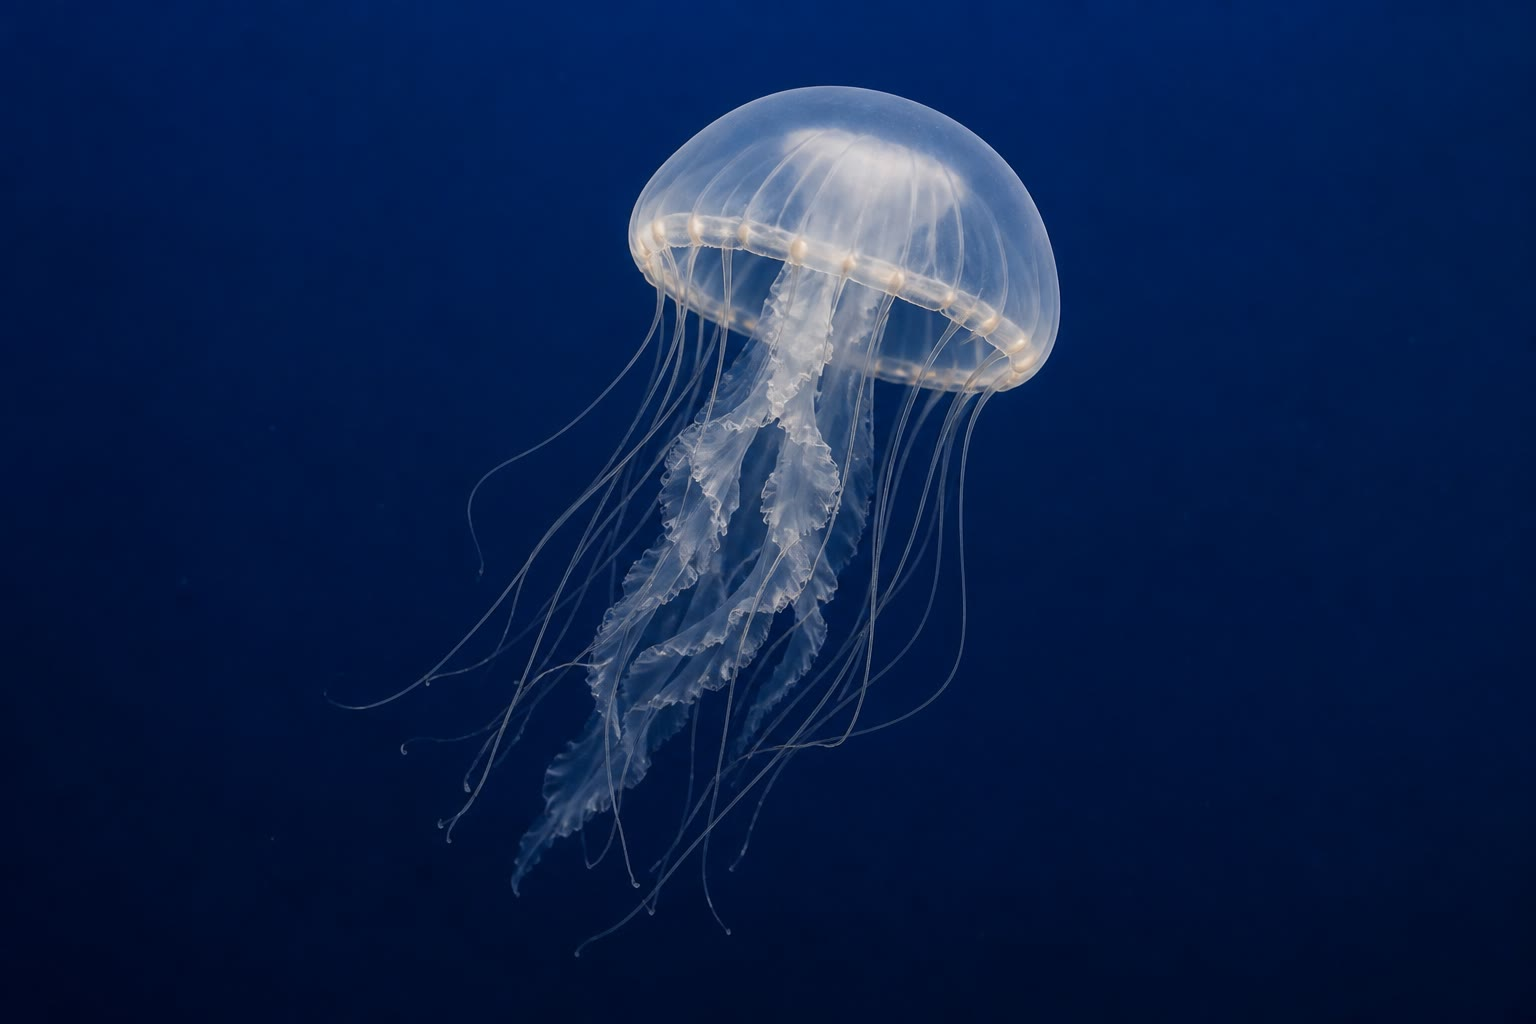
\includegraphics[width=0.46\linewidth]{images/book5/ai/b5-17-jellyfish.jpg}\hspace{0.04\linewidth}
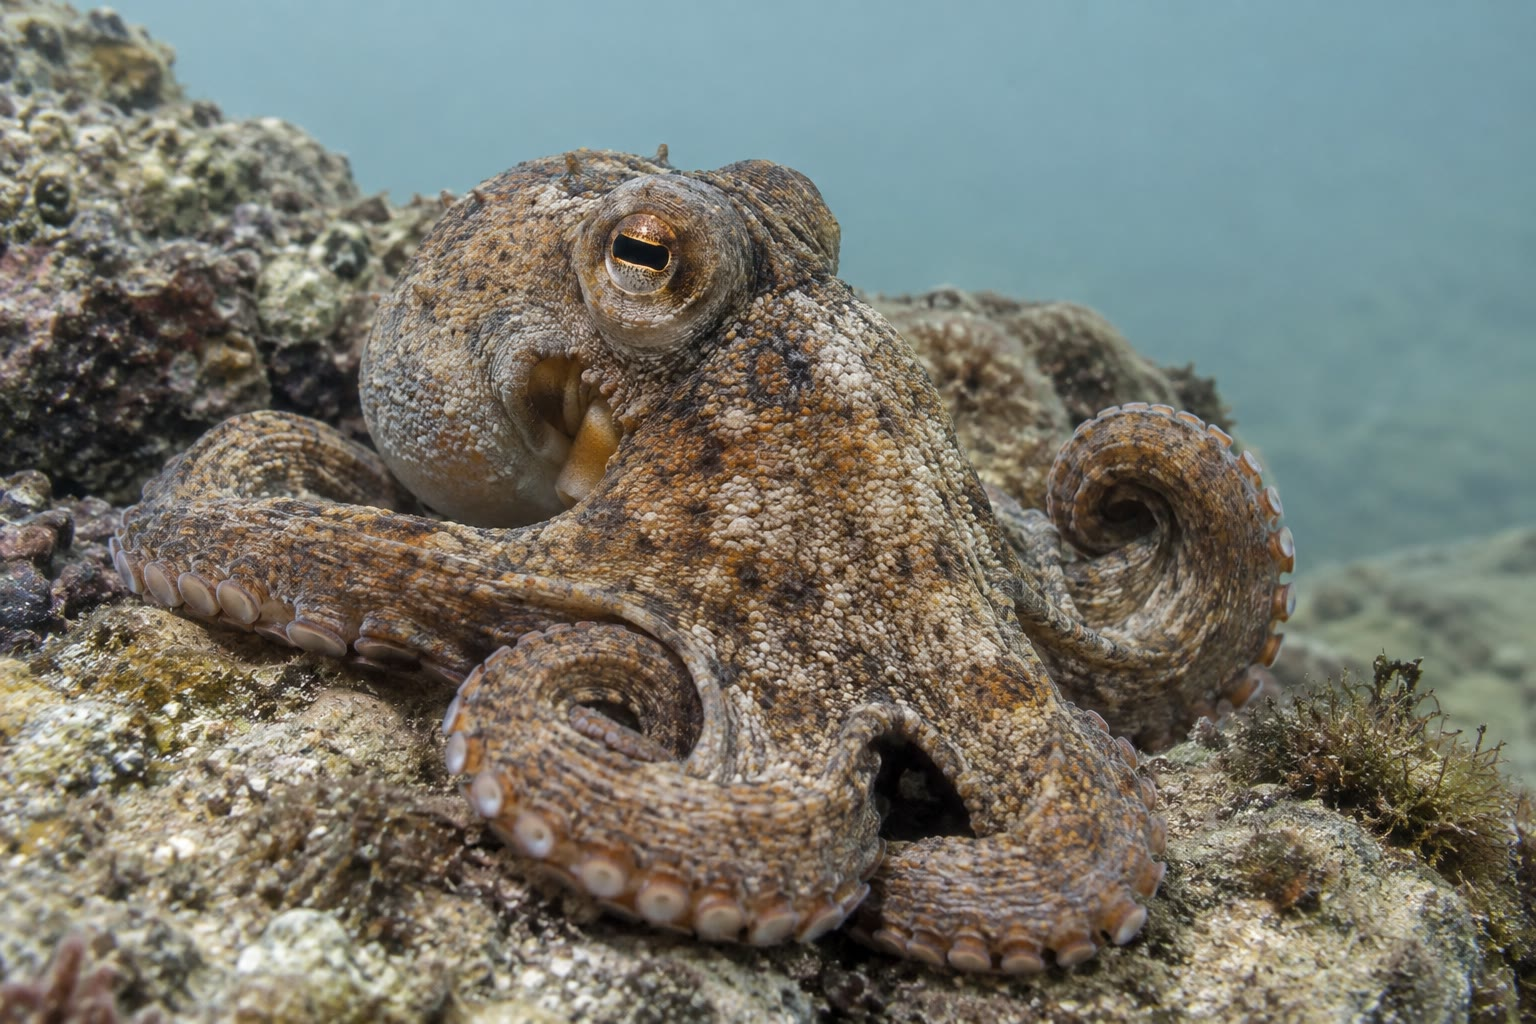
\includegraphics[width=0.46\linewidth]{images/book5/ai/b5-17-octopus.jpg}

{\small Dua cara menata neuron. Kiri: seekor ubur-ubur, yang \omterm{def:b3:nervous-systems:comparative}{jala sarafnya}
dan cincin tepinya menyelaraskan renangnya tanpa otak. Kanan: seekor
gurita, dengan setengah miliar neuron, kebanyakan di dalam lengannya, dan
otak terbesar di antara hewan tak bertulang belakang mana pun.}
\end{omfigure}

\begin{remark}[Untuk apa sebuah sistem saraf]\label{rem:b3:nervous-systems:for}
Tumbuhan, jamur, dan bunga karang tidak punya satu pun; seekor hewan yang
bergerak memerlukannya, dan perumitan sistem saraf menjejaki tuntutan gerakan,
penginderaan dari kejauhan, dan peramalan apa yang akan terjadi berikutnya.
\omterm{thm:b3:nervous-systems:cable}{Persamaan kabelnya} menetapkan fisikanya --- seberapa jauh dan seberapa cepat
sebuah isyarat mengembara bagi sebuah garis tengah dan isolasi tertentu;
anggaran tenaganya menetapkan ekonominya; dan di dalam batas itu neuron yang
sama, yang disusun sebagai jala, \omterm{def:b3:nervous-systems:comparative}{ganglion}, atau sebuah korteks, menghasilkan
denyut seekor ubur-ubur, penyamaran seekor gurita, atau kalimat ini. Kedua bab
berikutnya mengambil ujung masukannya dan penyimpanannya: bagaimana indra
mengubah dunia menjadi lecutan, dan bagaimana sinapsis berubah sehingga
dunianya, sekali dijumpai, teringat.
\end{remark}

\section{Latihan}

\begin{exercise}[$\star$]\label{exo:b3:nervous-systems:1}
Namailah keempat jenis \omterm{def:b3:nervous-systems:cells}{glia} dan satu fungsi masing-masing, lalu katakanlah yang
mana dua yang membuat \omterm{def:b3:nervous-systems:cells}{mielin} dan di mana.
\end{exercise}

\begin{exercise}[$\star$]\label{exo:b3:nervous-systems:2}
Apa yang dimungkinkan pewarna Golgi, apa yang disimpulkan Cajal darinya,
dan apa yang disimpulkan Golgi? Mana yang benar, dan bagaimana hal itu diputuskan?
\end{exercise}

\begin{exercise}[$\star$]\label{exo:b3:nervous-systems:3}
Perikanlah \omterm{def:b3:nervous-systems:circuits}{lengkung refleks} sentakan lutut lalu jelaskanlah mengapa ia memakan
hanya \qty{30}{ms} sedangkan sebuah tendangan sukarela memakan sepuluh kali lebih lama.
\end{exercise}

\begin{exercise}[$\star$]\label{exo:b3:nervous-systems:4}
Sebutkanlah pengaruh simpatis dan parasimpatis pada jantung,
biji mata, usus, dan saluran napas, serta penghantar yang dipakai tiap bagian
pada sasarannya.
\end{exercise}

\begin{exercise}[$\star\star$]\label{exo:b3:nervous-systems:5}
Hitunglah \omterm{thm:b3:nervous-systems:cable}{tetapan panjang} sebuah akson \qty{1}{\micro m} dengan $R_{m}
= \qty{1e4}{\ohm.cm^2}$ dan $R_{i} = \qty{100}{\ohm.cm}$, lalu
bagian isyarat yang tersisa sesudah \qty{2}{mm}. Garis tengah berapa yang akan
melipatduakan $\lambda$?
\end{exercise}

\begin{exercise}[$\star\star$]\label{exo:b3:nervous-systems:6}
Sebuah akson indra \qty{12}{\micro m} berjalan \qty{1.2}{m} dari jari kaki ke
sumsumnya, dan sebuah akson motorik \qty{15}{\micro m} kembali. Dengan
\qty{6}{m/s} tiap mikrometer dan \qty{0.5}{ms} tiap sinapsis, taksirlah
selang waktu minimum sebuah refleks penarikan tulang belakang dengan satu \omterm{def:b3:nervous-systems:cells}{interneuron}.
Berapa lama ia akan memakan waktu dengan akson tak bermielin bergaris tengah sama pada
$v = 1.1\sqrt{d}$?
\end{exercise}

\begin{exercise}[$\star\star$]\label{exo:b3:nervous-systems:7}
Dengan memakai anggaran otaknya dari
\cref{prop:b3:nervous-systems:barrier-budget}, taksirlah berapa banyak ATP yang
dapat dibelanjakan sebuah neuron tiap detik, dan, bila sebuah lecutan dengan
sinapsisnya berongkos $2\times 10^{9}$ ATP, laju penyalaan rata-rata yang
diizinkan anggarannya. Apa yang diramalkan hal ini tentang sandinya?
\end{exercise}

\begin{exercise}[$\star\star$]\label{exo:b3:nervous-systems:8}
Jelaskanlah mengapa sebuah \omterm{prop:b3:nervous-systems:cpg}{pengayun setengah-pusat} memerlukan kelelahan (atau
proses lambat lain) untuk mengayun, dan apa yang akan terjadi dengan dua neuron
yang saling menghambat yang tidak pernah lelah.
\end{exercise}

\begin{exercise}[$\star\star$]\label{exo:b3:nervous-systems:9}
Penghadang darah--otak menyingkirkan dopamin yang merupakan produk L-dopa tetapi
memasukkan L-dopa. Jelaskanlah bagaimana hal ini dimanfaatkan pada penyakit
Parkinson dan mengapa \omterm{def:b3:adaptive-immunity:antibody}{antibodi} terhadap protein otak sukar dihantarkan.
\end{exercise}

\begin{exercise}[$\star\star\star$]\label{exo:b3:nervous-systems:10}
Turunkanlah bentuk bergantung-waktu \omterm{thm:b3:nervous-systems:cable}{persamaan kabelnya}, $\lambda^{2}\,\partial^{2}
V/\partial x^{2} = \tau\,\partial V/\partial t + V$, dengan menambahkan
arus kapasitif ke arus selaputnya, lalu tunjukkanlah bahwa
penyelesaian keadaan mantap teoremanya menyusul. (Nyatakanlah bentuknya;
menyelesaikannya tidak diminta.) Mengapa nisbah $\lambda/\tau$ sebuah laju?
\end{exercise}

\begin{exercise}[$\star\star\star$]\label{exo:b3:nervous-systems:11}
Sebuah akson raksasa cumi-cumi \qty{500}{\micro m} menghantar pada \qty{25}{m/s}.
Dengan memakai $v \propto \sqrt{d}$, garis tengah akson tak bermielin berapa yang
diperlukan bagi \qty{100}{m/s}? Hitunglah luas penampangnya lalu bandingkanlah
dengan akson bermielin \qty{20}{\micro m} yang mencapainya. Apa yang
disiratkan hal ini tentang cacah serat cepat yang dapat diusung sebuah saraf, dan tentang
evolusi \omterm{def:b3:nervous-systems:cells}{mielin}?
\end{exercise}

\begin{exercise}[$\star\star\star$]\label{exo:b3:nervous-systems:12}
Massa otak berskala sebagai $M_{\text{tubuh}}^{0.75}$ di seluruh mamalia. Seekor
mencit \qty{30}{g} punya otak \qty{0.4}{g}. Ramalkanlah massa otak seekor
mamalia \qty{70}{kg} pada garisnya, bandingkanlah dengan \qty{1350}{g} manusia,
lalu bahaslah mengapa cacah neuron korteks alih-alih massa otaknya yang menjadi
padanan yang lebih baik bagi kemampuan kognitifnya.
\end{exercise}

\section{Soal: Merangkai Sebuah Tubuh}

\begin{problem}[{Soal akhir pekan --- perangkaian sebuah tubuh yang diongkosi dalam
tetapan panjang, milidetik, dan watt: angka kabel sebuah
dendrit dan dua akson, selang waktu sebuah refleks dari jari kaki ke sumsumnya dan
kembali, tenaga yang dapat dibayar otaknya tiap lecutan, serta penskalaan
otak di berbagai hewan, berakhir pada tetapan panjangnya, selang waktu refleksnya,
dan laju penyalaan rata-rata yang dapat dibayar sebuah otak}]
\label{pb:b3:nervous-systems:1}
Data: $R_{m} = \qty{2e4}{\ohm.cm^2}$, $R_{i} = \qty{100}{\ohm.cm}$,
$C_{m} = \qty{1}{\micro F/cm^2}$. Laju bermielin \qty{6}{m/s} tiap
mikrometer; tak bermielin $v = 1.1\sqrt{d}$ m/s dengan $d$ dalam
mikrometer; penundaan sinapsis \qty{0.5}{ms}. Otak: \qty{20}{W},
$8.6\times 10^{10}$ neuron, $10^{14}$ sinapsis, ATP \qty{50}{kJ/mol};
sebuah lecutan berongkos $4\times 10^{8}$ ATP dan tiap penularan sinapsis
$2\times 10^{4}$ ATP; sebuah neuron punya \num{7000} sinapsis. Penskalaan:
$M_{\text{otak}} = a\,M_{\text{tubuh}}^{0.75}$ dengan seekor mencit \qty{30}{g}
yang berotak \qty{0.4}{g}.

\medskip
\noindent\textbf{Bagian I --- Kabel.}
\begin{enumerate}
  \item Hitunglah $\lambda$ bagi dendrit \qty{1}{\micro m} dan
        \qty{4}{\micro m}, serta $\tau$.
  \item Sebuah sinapsis \qty{300}{\micro m} dari soma pada dendrit
        \qty{1}{\micro m} menghasilkan \qty{5}{mV} setempat. Berapa yang
        tiba di somanya? Pada dendrit \qty{4}{\micro m}?
  \item Jelaskanlah mengapa sebuah neuron dapat membobot masukannya menurut di
        mana pada pohonnya masukan itu mendarat, dan mengapa masukannya harus tiba
        dalam sekitar $\tau$ agar terjumlahkan.
  \item Hitunglah laju sebuah akson bermielin \qty{10}{\micro m},
        dan sebuah akson tak bermielin bergaris tengah sama. Garis tengah berapa
        akson tak bermielin yang akan menyamai yang bermielin?
  \item Luas penampang akson \qty{10}{\micro m} dan
        akson tak bermielin yang setara. Berapa banyak akson bermielin yang muat di
        dalam ruang satu akson tak bermielin yang setara?
  \item Sebuah penyakit pelucut \omterm{def:b3:nervous-systems:cells}{mielin} membuang \omterm{def:b3:nervous-systems:cells}{mielin} dari sebuah akson
        \qty{10}{\micro m} sepanjang \qty{2}{cm}. Taksirlah penundaan tambahan
        sepanjang bentangan itu bila ia menghantar sebagai akson tak bermielin
        bergaris tengah itu, lalu katakanlah mengapa hantarannya dapat gagal sama sekali.
\end{enumerate}

\medskip
\noindent\textbf{Bagian II --- Selang waktu.}
\begin{enumerate}[resume]
  \item Sebuah jari kaki menyentuh permukaan panas. Akson indranya (\qty{10}{\micro m},
        \qty{1.2}{m}) mencapai sumsumnya, satu \omterm{def:b3:nervous-systems:cells}{interneuron}, lalu sebuah akson motorik
        (\qty{15}{\micro m}, \qty{1.1}{m}) kembali ke tungkainya. Berapa selang waktu
        minimum penarikannya?
  \item Isyaratnya juga berjalan naik sebuah akson \qty{10}{\micro m}
        sejauh \qty{0.6}{m} ke otaknya lalu menembus dua sinapsis lagi sebelum
        nyerinya terasa. Kapan nyerinya terasa relatif terhadap penarikannya?
  \item Sebuah serat nyeri tidak bermielin, \qty{1}{\micro m}. Berapa lama
        isyaratnya memakan waktu untuk menempuh \qty{1.8}{m} ke otaknya? Jelaskanlah
        kedua fase nyeri dari jari kaki yang tersandung.
  \item Tungkai seekor jerapah \qty{2}{m} lebih panjang. Hitunglah ulang selang waktu
        refleksnya lalu berilah ulasan tentang masalah ukuran.
  \item Sentakan lutut bersifat monosinaptik, \qty{30}{ms} pada orang dewasa. Dengan
        memakai \qty{0.8}{m} tiap arah pada \qty{80}{m/s}, satu sinapsis dan sebuah
        sambungan saraf--otot (\qty{1}{ms}), serta \qty{5}{ms} bagi
        ototnya untuk membangun gaya, pertanggungjawabkanlah \qty{30}{ms} itu.
  \item Akson bayi baru lahir belum bermielin. Jelaskanlah mengapa refleksnya
        lambat dan gerakannya tak terselaras, dan apa yang diubah pemielinan
        selama dua tahun pertamanya.
\end{enumerate}

\medskip
\noindent\textbf{Bagian III --- Anggarannya.}
\begin{enumerate}[resume]
  \item Ubahlah \qty{20}{W} menjadi ATP tiap detik, dan menjadi ATP tiap neuron
        tiap detik.
  \item Sebuah neuron menyalakan satu lecutan: ia berongkos $4\times 10^{8}$ ATP
        sendiri lalu menggerakkan \num{7000} sinapsis pada $2\times 10^{4}$ masing-masing.
        Berapa ongkos total satu lecutan dengan akibatnya?
  \item Laju penyalaan rata-rata berapa yang dapat ditopang anggarannya bila
        semuanya dipakai untuk lecutan? Bila separuhnya pergi ke ongkos istirahat?
  \item Neuron korteks menyala pada sekitar \qty{1}{Hz} rata-rata. Berapa
        bagian anggarannya yang demikian, dan apa yang disiratkannya tentang
        bagaimana keterangannya disandi?
  \item Sebuah otak yang menyalakan tiap neuronnya pada \qty{50}{Hz} akan memerlukan
        berapa watt? Bandingkanlah dengan \qty{100}{W} seluruh tubuhnya.
  \item Glukosa memasok otaknya pada \qty{5}{g/h}. Berapa watt itu
        (\qty{16}{kJ/g})? Cukupkah, dan apa yang terjadi pada
        kesadarannya dalam hitungan detik sesudah pasokannya gagal?
\end{enumerate}

\medskip
\noindent\textbf{Bagian IV --- Penskalaan.}
\begin{enumerate}[resume]
  \item Temukanlah $a$ dari mencitnya, lalu ramalkanlah massa otak seekor
        mamalia \qty{70}{kg} dan seekor gajah \qty{5000}{kg} pada
        garisnya.
  \item Nilai sebenarnya: manusia \qty{1350}{g}, gajah \qty{4800}{g}.
        Hitunglah nisbah tiap spesies terhadap ramalannya (yakni
        hasil bagi \omterm{def:b3:nervous-systems:comparative}{ensefalisasi}).
  \item Otak gajahnya punya $2.6\times 10^{11}$ neuron tetapi
        $5.6\times 10^{9}$ di dalam korteksnya; manusianya $8.6\times 10^{10}$
        dan $1.6\times 10^{10}$. Di mana neuron gajahnya, dan
        apa yang disarankannya tentang apa yang dikerjakan korteks?
  \item Volume sebuah neuron tumbuh seiring panjang aksonnya, sehingga otak yang
        lebih besar punya neuron yang lebih besar dan lebih jarang. Jelaskanlah mengapa
        melipatduakan massa otaknya tidak melipatduakan cacah neuronnya, dan mengapa
        primata, yang neuronnya tetap kecil sementara otaknya tumbuh, memperoleh
        lebih banyak neuron tiap gram daripada hewan pengerat.
  \item Seekor gurita punya $5\times 10^{8}$ neuron, dua pertiganya di dalam lengannya.
        Usulkanlah apa yang dapat dan tidak dapat dilakukan sebuah lengan tanpa otaknya, dan
        satu percobaan untuk mengujinya.
  \item Nematoda \emph{C.~elegans} punya $302$ neuron dan sekitar
        \num{7000} sinapsis seluruhnya, yang tiap satunya dipetakan. Bandingkanlah
        sinapsis tiap neuronnya dengan angka manusia, lalu katakanlah apa yang dapat dan
        tidak dapat dikatakan sebuah diagram perangkaian yang lengkap tentang tingkah laku.
  \item Ringkaslah: \omterm{thm:b3:nervous-systems:cable}{tetapan panjang} dendrit \qty{1}{\micro m}
        (pertanyaan~1), selang waktu refleks penarikannya (pertanyaan~7), dan
        laju penyalaan rata-rata yang diizinkan anggaran otaknya dengan separuh
        tenaganya untuk lecutan (pertanyaan~15).
\end{enumerate}
\end{problem}
